
\section{两个态射相等之处，与「既约到分离」定理}

我们在 \S7.5 引入\trRationalMap{}时曾经许诺：在良好的情形下，一个\trRationalMap{}拥有一个「最大的\trDomainOfDefinition」。现在，我们终于可以把「良好的情形」说精确了，办法正是「既约到分离」定理~11.3.2。我们首先引入一个重要的结果，让「源与目标皆相同的两个\trMorphism{}『相等』之处」这一说法有了确切含义。

\textbf{11.3.A.（有用的练习：两个态射相等之处）}\quad 设 $\pi\colon X\to Y$ 与 $\pi'\colon X\to Y$ 是某个概形 $Z$ 上的两个\trMorphism。
\[
\begin{tikzcd}[row sep=2.2em]
X \ar[rr, bend left=17, "\pi"] \ar[rr, bend right=17, "\pi'"'] \ar[dr] & & Y \ar[dl] \\
& Z &
\end{tikzcd}
\]
现在我们可以给「$\pi$ 与 $\pi'$ 相等之处」这一说法以确切含义了；特别地，还可以谈这样一个事实：存在一个最大的局部闭子概形使二者在其上相等——而当 $Y$ 在 $Z$ 上\trSeparated{}时，它还是闭的。设 $\mu\colon W\to X$ 是某个\trMorphism（不必假设它是局部闭嵌入）。若 $\pi\circ\mu=\pi'\circ\mu$，就说 $\pi$ 与 $\pi'$ 在 $\mu$ 上相等。证明：存在一个局部闭子概形 $\iota\colon\mathsf{V}\hookrightarrow X$，使 $\pi$ 与 $\pi'$ 在其上相等，并且任何使 $\pi$ 与 $\pi'$ 在其上相等的\trMorphism{} $\mu\colon W\to X$ 都唯一地穿过 $\iota$ 分解，也就是说，存在唯一的 $j\colon W\to\mathsf{V}$ 使 $\mu=\iota\circ j$。再证明：若 $Y\to Z$ 是\trSeparated{}的，则 $\iota\colon\mathsf{V}\hookrightarrow X$ 是一个\trClosedEmbedding。

提示：把 $\mathsf{V}$ 定义为如下的\trFiberProduct{}：
\[
\begin{tikzcd}[row sep=2.6em, column sep=3.4em]
\mathsf{V} \ar[r] \ar[d] & Y \ar[d, "\delta"] \\
X \ar[r, "{(\pi,\pi')}"'] & Y\times_Z Y.
\end{tikzcd}
\]
由于 $\delta$ 是\trLocallyClosedEmbedding，$\mathsf{V}\to X$ 亦然。于是，若 $\mu\colon W\to X$ 是任一满足 $\pi\circ\mu=\pi'\circ\mu$ 的\trMorphism，则 $\mu$ 穿过 $\mathsf{V}$。

两个映射相等之处可以不\trReduced{}，这不该令人吃惊：考虑从 $\mathbb{A}^1_k$ 到其自身的两个映射 $\pi(x)=0$ 与 $\pi'(x)=x^2$。它们在 $x=0$ 处相等，但情形（按 $\epsilon$ 的标准来衡量）还要更好——它们甚至应当在 $\Spec k[x]/(x^2)$ 上相等。\footnote{译注：epsilonically 系作者生造的词，把幂零增厚戏称为「$\epsilon$ 层次」的分辨本领：能分辨到 $\Spec k[x]/(x^2)$，就比只分辨底层点又精确了一步。}

\textbf{11.3.1.}\ \emph{小注记。}\quad (i) 在上一道练习中，我们用\trUniversalProperty{}描述了 $\mathsf{V}\to X$。若径以之为定义，那么 $\mathsf{V}$ 是 $X$ 的局部闭子概形——甚至它存在与否——都不是先验显然的。

(ii) \trhWarning{}：考虑 $\Spec\mathbb{C}$ 到自身、在 $\Spec\mathbb{R}$ 之上的两个映射：恒同与\trComplex\trConjugate。二者都是从点到点的映射，然而尽管作为集合的映射相等，它们却不相等。（若你不信它们作为\trMorphism{}并不相等，下面这话或许有帮助：经过\trBaseChange{} $\Spec\mathbb{C}\to\Spec\mathbb{R}$ 之后，它们连作为集合的映射都不相等了。）

(iii) 更一般地，$\pi$ 与 $\pi'$ 相等的（集合论）轨迹可以这样解读：$\pi$ 与 $\pi'$ 在点 $p$ 处相等，是指 $\pi(p)=\pi'(p)$，且由此给出的两个\trResidueField{}之间的映射相同。（你也许会乐于把这件事当作一道练习想个明白。\footnote{原书此处作（You may enjoying thinking），当系「enjoy」之误，径改。——译者注}）

\textbf{11.3.B.（练习：$\overline{K}$-\trVariety{}由闭点上的映射决定）}\quad 设 $\pi\colon X\to Y$ 与 $\pi'\colon X\to Y$ 是两个 $\overline{K}$-\trVariety{}之间的\trMorphism，它们在闭点的层面上相同（也就是说，对每个\trClosedPoint{} $p\in X$ 都有 $\pi(p)=\pi'(p)$）。证明：$\pi=\pi'$。（这蕴含：从「$\overline{K}$ 上的经典簇」这一\trCategory——我们不在此定义它——到 $\overline{K}$-\trScheme{}的\trCategory{}的\trFunctor{}是\trFullyFaithful{}的。你能把它恰当地推广到非\trAlgClosedField{}的情形吗？）

\textbf{11.3.C.（较不重要的练习）}\quad 证明：原点加倍了的\trAffineLine{} $X$（例~4.4.5）不是\trSeparated{}的，办法是找出两个\trMorphism{} $\pi\colon W\to X$、$\pi'\colon W\to X$，使得二者的「相等定义域」不是\trClosedSubscheme（对比\mbox{命题~11.2.1(b)}）。（\mbox{练习~11.2.I}已在上文给出另一个论证；\mbox{练习~13.7.C}将给出一个花哨的论证。）

现在我们来到本节的中心结果。

\textbf{11.3.2.\ 「既约到分离」定理}（Reduced-to-Separated Theorem）\textbf{。}\ ——\ \emph{从一个\trReduced\trScheme{}到一个\trSeparated{}的 $S$-\trScheme{}的两个 $S$-态射 $\pi\colon\mathsf{U}\to Z$、$\pi'\colon\mathsf{U}\to Z$，若在 $\mathsf{U}$ 的一个\trDense\trOpenSubset{}上相等，则二者相同。}

\emph{证明。}\ 令 $\mathsf{V}$ 为 $\pi$ 与 $\pi'$ 相等之处。它是 $\mathsf{U}$ 的一个\trClosedSubscheme（由\mbox{练习~11.3.A}），并且含有一个稠密开集。但既约概形 $\mathsf{U}$ 的\trClosedSubscheme{}之中，底集合稠密者唯有 $\mathsf{U}$ 自身。（你看出最后这句话为什么成立吗？若去掉既约性假设，你能给出反例吗？）\hfill$\square$

\textbf{11.3.3.}\quad \emph{推论~1。}\ 于是（由于 $X$ 既约、$Y$ 分离），若有两个从 $X$ 的开子集出发、到 $Y$ 的\trMorphism，比如说 $\pi\colon\mathsf{U}\to Y$ 与 $\pi'\colon\mathsf{V}\to Y$，并且它们在 $\mathsf{U}\cap\mathsf{V}$ 的一个稠密开子集 $Z$ 上相等，那么它们必在 $\mathsf{U}\cap\mathsf{V}$ 上相等。

\emph{推论~2。}\ 一个\trRationalMap{}拥有一个最大的\trDomainOfDefinition{}——$\pi\colon\mathsf{U}\dashrightarrow Y$ 在其上是一个\trMorphism{}——它就是全部\trDomainOfDefinition{}之并。特别地，\trReduced\trScheme{}上的\trRationalFunction{}拥有一个最大的\trDomainOfDefinition。例如，由 $(x,y)\mapsto[x,y]$ 给出的\trRationalMap{} $\mathbb{A}^2_k\dashrightarrow\mathbb{P}^1_k$，其\trDomainOfDefinition{}为 $\mathbb{A}^2_k\setminus\{(0,0)\}$（参看 \S7.5.3）。这在部分程度上推广了\trLocally\trNoetherian{}概形上\trRationalFunction{}之定义域的观念（定义~6.6.36）。\trDomainOfDefinition{}的补集称为\textbf{\trIndeterminacyLocus}（indeterminacy locus；这一说法早先已在 \S6.6.36 中使用过），它的点有时被称为该\trRationalMap{}的\textbf{\trFundamentalPoint{}}（fundamental points），不过我们不会使用这些说法。（我们将在\mbox{练习~22.4.L}中看到：到\trProjectiveScheme{}的\trRationalMap{}可以通过「胀开」一个概形论版本的不定性轨迹，升级为一个名副其实的\trMorphism。）

\textbf{11.3.D.（练习）}\quad 证明：若放弃源的既约性或目标的分离性，「既约到分离」定理~11.3.2 便不成立。这里给出几种可能。对于第一种，考虑从 $\Spec k[x,y]/(y^2,xy)$ 到 $\Spec k[t]$ 的两个映射，其中 $\pi$ 由 $t\mapsto x$ 给出，$\pi'$ 由 $t\mapsto x+y$ 给出；$\pi$ 与 $\pi'$ 在由 $y=0$ 切出的\trClosedSubscheme{}上相等。对于第二种，考虑从 $\Spec k[t]$ 到原点加倍了的\trAffineLine{}的两个映射，其一映入「上半」，另一映入「下半」。这两个\trMorphism{}在稠密开集 $D(t)$ 上相等；见图~\ref{fig:nonseparated-agreement}。

\begin{figure}[htbp]
\centering
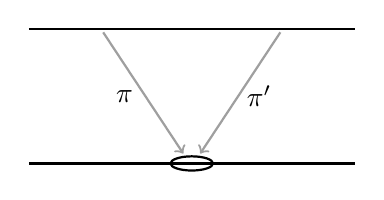
\begin{tikzpicture}[scale=0.9,line width=0.8pt]
  \draw (0,1.9) -- (4.6,1.9);
  \draw (0,0) -- (4.6,0);
  \draw[gray!75,->] (1.05,1.85) -- (2.18,0.14);
  \draw[gray!75,->] (3.55,1.85) -- (2.42,0.14);
  \node at (1.35,0.95) {$\pi$};
  \node at (3.25,0.95) {$\pi'$};
  \draw (2.3,0) ellipse (0.3 and 0.1);
\end{tikzpicture}
\caption{到一个非\trSeparated{}\trScheme{}的两个不同映射在一个稠密开集上相等（见练习 11.3.D）。依原书手绘图重绘。}\label{fig:nonseparated-agreement}
\end{figure}

\textbf{11.3.4.}\ \emph{有理映射的图像。}\quad（\emph{\trMorphism}的图像已在 \S11.2.5 中定义。）若 $X$ 既约而 $Y$ \trSeparated{}，则如下定义\trRationalMap{} $\pi\colon X\dashrightarrow Y$ 的\textbf{图像 $\Gamma_\pi$}（graph）。任取这个\trRationalMap{}的一个代表 $(\mathsf{U},\pi')$（于是 $\pi'\colon\mathsf{U}\to Y$ 是一个\trMorphism）。令 $\Gamma_\pi$ 为 $\Gamma_{\pi'}\hookrightarrow\mathsf{U}\times Y\hookrightarrow X\times Y$ 的\trSchemeTheoretic{}闭包，其中第一个映射是\trClosedEmbedding（命题~11.2.6），第二个映射是\trOpenEmbedding。这里的积应当在你所工作的\trCategory{}中取。例如，如果你处理的是 $k$-\trScheme，纤维积就应当取在 $k$ 上。

\textbf{11.3.E.（练习）}\quad 证明：\trRationalMap{} $\pi\colon X\dashrightarrow Y$ 的图像不依赖于 $\pi$ 之代表的选取。提示：设 $\xi'\colon\mathsf{U}\to Y$ 与 $\xi\colon\mathsf{V}\to Y$ 是 $\pi$ 的两个代表。化归到 $\mathsf{V}$ 是 $\pi$ 的\trDomainOfDefinition（\S11.3.3）且 $\xi'=\xi|_{\mathsf{U}}$ 的情形。再化归到 $\mathsf{V}=X$ 的情形。证明同构 $\Gamma_\pi\cong X$ 与 $\Gamma_{\xi|_{\mathsf{U}}}\cong\mathsf{U}$。（评注：$Y$ 的分离性并不必要。）

类比\trMorphism{}的图像，下面这幅展示\trRationalMap{} $\pi$ 之图像的图示可能会有用（参看\cref{fig:graph-morphism}）。
\[
\begin{tikzcd}[row sep=3em, column sep=3.4em]
\Gamma_\pi \ar[hook, r, "\text{闭嵌入}"] & X\times Y \ar[dr, "\mathrm{pr}_2"] \ar[dl, "\mathrm{pr}_1"] \\
X \ar[u, dotted, "\Upsilon_\pi"'] \ar[rr, dashed, "\pi"] & & Y.
\end{tikzcd}
\]

\textbf{11.3.F.（练习：作为\trRationalMap{}之图像的仿射平面胀开）}\quad 考虑由 $(x,y)\mapsto[x,y]$ 给出的\trRationalMap{} $\mathbb{A}^2_k\dashrightarrow\mathbb{P}^1_k$。证明：这个\trRationalMap{}不能越过原点延拓。（\mbox{练习~7.5.J}中关于\trCremona{}变换的论证与此相类。）证明：这个\trRationalMap{}的图像正是\mbox{练习~10.3.F}所描述的那个\trMorphism（胀开）。（等我们在一般情形下定义胀开时，将会看到它们往往就是\trRationalMap{}的图像；见\mbox{练习~22.4.M}。）

\textbf{11.3.5.\ 变奏。}\quad 定理~11.3.2 那个短证明的种种变奏，可以给出其他有用的结果。\mbox{练习~11.3.B}便是一例。这里是另一例。

\textbf{11.3.G.（练习：到分离概形的映射越过\trEffectiveCartierDivisor{}至多只能以一种方式延拓）}\quad 设 $X$ 是一个 $Z$-\trScheme（不必\trReduced！），而 $Y$ 是一个\trSeparated{}的 $Z$-\trScheme。再设 $D$ 是 $X$ 上的一个\trEffectiveCartierDivisor。证明：任何一个 $Z$-\trMorphism{} $X\setminus D\to Y$ 至多只能以一种方式延拓为 $Z$-\trMorphism{} $X\to Y$。（提示：化归到 $X=\Spec A$ 而 $D$ 为 $t\in A$ 的\trVanishingScheme{}的情形。再化归到证明 $D(t)$ 在 $X$ 中的\trSchemeTheoreticImage{}是整个 $X$。为此可证 $A\to A_t$ 是单的。）

如 \S7.5.2 所述，只要 $X$ 带有\trAssociatedPoint，便可以定义从 $X$ 到任何 $Y$ 的\trRationalMap{}。「既约到分离」定理~11.3.2 可以推广到这一场合，如下。

\textbf{11.3.H.（练习：「相伴到分离」定理（Associated-to-Separated Theorem））}\quad 证明：从一个\trLocally\trNoetherian{}概形 $\mathsf{U}$ 出发、到一个\trSeparated{}的 $S$-\trScheme{} $Z$ 的两个 $S$-\trMorphism{} $\pi$ 与 $\pi'$，若在一个含有 $\mathsf{U}$ 的全部\trAssociatedPoint{}的开子集上相等，则二者相同。
